As covered in \sectionref{related}, the current leading methods in object detection are within the domain of deep learning. This chapter will cover the core concepts of deep learning which will include general architecture of \glspl{cnn}, typical layers and optimisation strategies. Also covered will be aspects of deep learning that are more specific to object detection with \glspl{cnn}.

\section{Convolutional Neural Networks}
\glspl{cnn} are an extension of artificial neural networks which have existed for decades. Neural networks consist of neurons that receive inputs and have learned parameters such that the input can be altered in some manner. In the neuron, the dot product is computed between the input and parameters \cite{cs321n}. For \glspl{cnn}, the key difference is the first input to the network is an image and the parameters in the neurons are filters which are trained to activate towards certain inputs. One of the first successful \gls{cnn} methods was LeNet for hand-written digit classification in 1989 \cite{lenet}. However, after this point, deep learning research became stagnant mostly due to the large amount of processing needed in training. The return of deep learning is often attributed to AlexNet in 2012 \cite{alexnet}, which gave significant improvements in image classification on ImageNet.
\\\\
The general architecture of a \gls{cnn} is shown in \figref{generalcnn}. The network takes an image as input, this can be a single channel as depicted in the figure or multiple such as an colour image. Convolutional operations with learned filters are applied to an area of the input image dependent on the filter size to produce an output at a given layer shown by the red dot. The size of the filters at a given layer constitutes the receptive field of that layer. For example, a 9$\times$9 filter has a larger receptive field than a 3$\times$3 filter to produce a given response. Each filter is individually trained and shown as the arrows leading to the dots. In the second convolutional layer is where the network starts to be considered deep. Again, convolutional operations are performed to produce an output. Depending on the architecture of the network many convolutional layers can be present, generally deeper networks are able to find richer abstract features for the given task. Finally the network may have a fully-connected layer that produces confidence scores. These scores can be used to determine how well an input image represents a given class for a classification problem.

\begin{figure}[H]
  \centering
    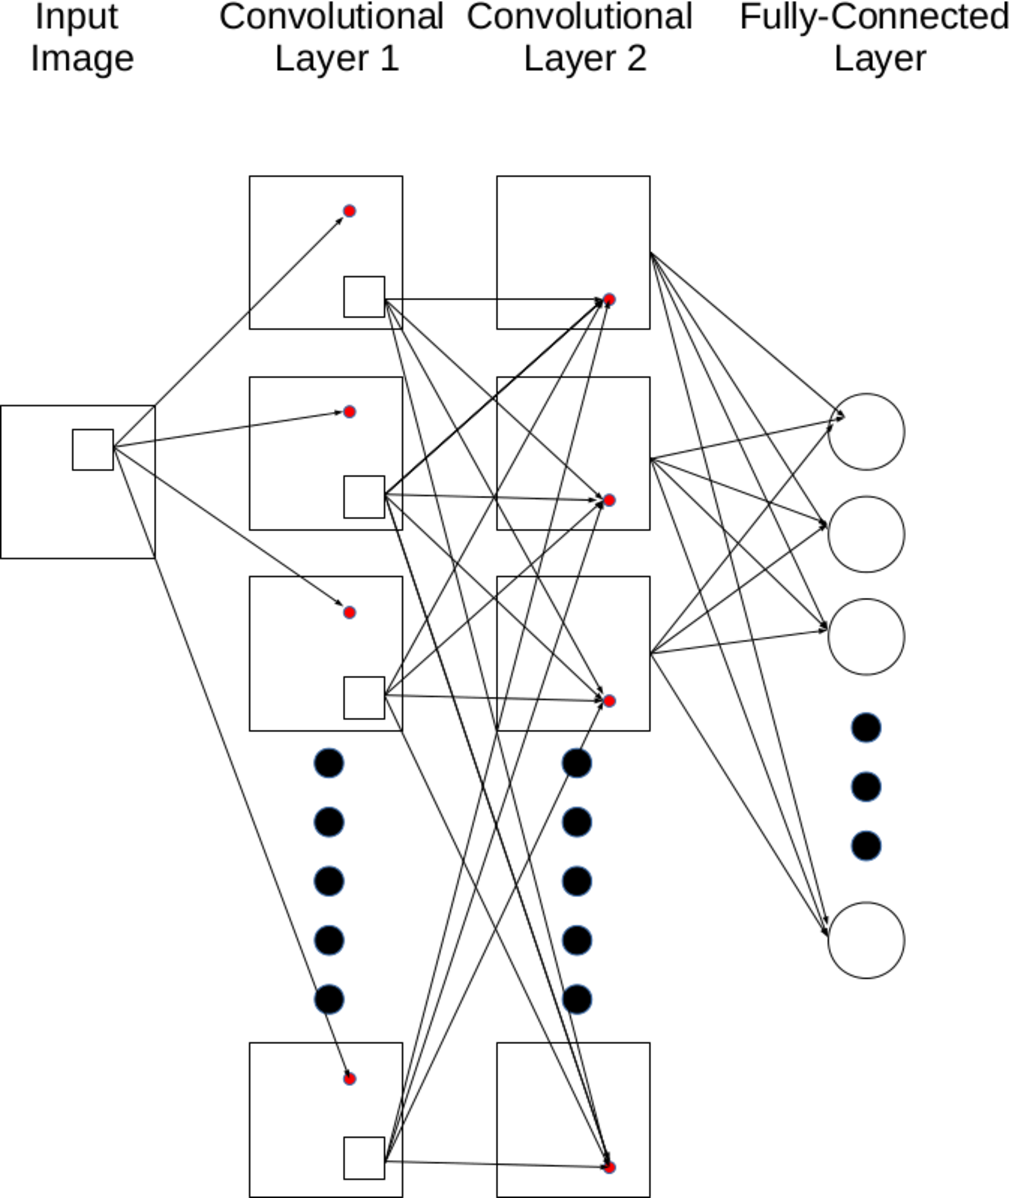
\includegraphics[width=0.6\textwidth]{Figs/Techanal/cnnarch.pdf}
      \caption{An example of a general \gls{cnn} with convolutional and fully-connected layers.}
    \label{fig:generalcnn}
\end{figure}

The activation function within a convolutional layer is another key aspect to neural networks. The activation layer is used to add non-linearity to the network and measures how well a given convolutional operation and associated bias fires for a patch in either the input image or a previous layer \cite{cs321n}. Typically activation functions output between 0 and 1 to represent this measurement. In earlier adaptations of \glspl{cnn} the a sigmoid activation function was popular to map the output of a convolutional layer between 0 and 1. However, most current \glspl{cnn} take advantage of the \glspl{relu} activation function. \gls{relu} is a simple thresholding function that maps negative outputs to 0 and positive outputs are kept unchanged.
\\\\
In order to learn the parameters in a \gls{cnn} an optimisation strategy is required. The training process is to minimise a loss function in respect the inputs. Typically the learning is done through gradient descent with backpropgation \cite{cs321n}. The intuition here is to update parameters after each forward iteration such that the loss calculated between input samples and their labels is decreased. Generally for each forward pass the loss is calculated as the average loss over a mini-batch of samples. This is both more efficient and produces a less stochastic learning process. Once the loss is found the gradient indicates which direction to update parameters and this information is backpropagated right through to the initial parameters.
\\\\
A key aspect of training \glspl{cnn} is how the parameters in a network are initialised. Poor initialisation of parameters can make the training process slow or impossible if the initial operations fire the activation functions too violently. Common approaches to initialisation include sampling the weights from a Gaussian distribution and setting all biases to zero. Other alternative dynamic approaches do exist, such as Xavier initialisation \cite{xavier}. In this case the architecture of the network is measured, such as number of filters in a layer, and weights are sampled according to this information. Another initialisation method is fine-tuning parameters from a pre-trained network. A pre-trained network is typically trained on a large set of data and has learnt parameters to that given task, then by updating the parameters they can be changed towards a new task. This can provide a number of benefits. Firstly, the amount of training time can be drastically reduced as strong general parameters have already been learned. Also, if the amount of training data is sparse, fine-tuning can aid such that the risk of overfitting is reduced.
